\chapter{Studies of environmental noise during O3}\label{ch:noise-studies}

\ac{O3} was preceded by an engineering run (ER13), a month-long period during with the interferometer is operational at low-noise levels but not observing \ac{GW} events, to provide time for detector commissioning and noise studies.
The main injection campaigns used to measure coupling for all PEM sensors are performed during these engineering runs.
A mid-run commissioning break ER14 took place in the month of October of 2019, during which some of the most crucial coupling measurements were repeated.
Although the observing run does not end with an engineering run, some time is still made for end-of-run commissioning that assesses changes in detector performance, including PEM noise studies, before the instruments are finally shut down for major upgrades.
The pre- and post-O3 campaigns are summarized in Table~\ref{tab:noise-campaigns}.
There were fewer post-O3 injections due to the premature termination of O3 in the wake of the COVID-19 pandemic.

\begin{table}[htb]
	\caption{Number of injections performed at each station and for each injection type throughout the pre-, and post-O3 injection campaigns.}
	\label{tab:noise-campaigns}
	\begin{tabular}{|c|ccccc|}
		\hline
		& Station & Magnetic & Magnetic & Vibrational & Vibrational \\
		& & (comb) & (broadband) & (acoustic) & (shaker) \\
		\hline
		LHO & Corner & 16 & 10 & 11 & 63 \\
		\multirow{2}{*}{Pre-O3} & End-X & 9 & 0 & 6 & 7 \\
		& End-Y & 9 & 0 & 9 & 14 \\
		\hline
		LHO & Corner & 10 & 2 & 11 & 0 \\
		\multirow{2}{*}{Post-O3} & End-X & 4 & 0 & 4 & 0 \\
		& End-Y & 9 & 0 & 5 & 0 \\
		\hline
		LLO & Corner & 7 & 3 & 14 & 0 \\
		\multirow{2}{*}{Pre-O3} & End-X & 3 & 0 & 2 & 0 \\
		& End-Y & 4 & 0 & 4 & 0 \\
		\hline
		LLO & Corner & 0 & 5 & 0 & 0 \\
		\multirow{2}{*}{Post-O3} & End-X & 0 & 3 & 0 & 0 \\
		& End-Y & 0 & 4 & 0 & 0 \\
		\hline
	\end{tabular}

\end{table}


\section{Evaluation of coupling functions}\label{sec:evaluation-of-cf}

Before discussing results of injection studies and coupling function measurements in \ac{O3}, it is necessary that we take a moment to assess how well they estimate excess noise in the interferometer when the noise source is known to be the result of environmental coupling.
Of course, one could do this by applying coupling functions to a set of ``test'' injections, but this would require performing more injections, which as mentioned before is typically not feasible.
Furthermore, since the intention of the coupling functions is to estimate the impact of noise signals originating from a broad variety of sources, it make sense to use non-laboratory signals when evaluating coupling estimates.
Therefore, we use noise events not produced by injection equipment to evaluate how accurately the coupling functions recover the actual excess noise observed in the \ac{GW} strain data.

Thunderstorms are known to produce short-duration transients in the strain data at tens of Hz by exciting vibrational coupling associated with scattered light.
S190510g, a long-duration GW trigger observed while a thunderstorm was underway at LLO, overlapped many such noise artifacts throughout its 255-s time span.
We can rule out any astrophysical origins for these signals: they are observed by accelerometers at all stations with reasonable delays for sound propagation, they sound like thunder on the microphone channels, and they have the right frequency content and duration. One of the loud events was also consistent with the time put in by an operator for a loud thunder clap.
Figure~\ref{fig:evaluation-thunder} shows constant-Q transforms of one of these thunder noises as seen in the LLO strain channel as well as one of the End-Y accelerometers, where scattered light coupling was a dominant noise source.
Coupling functions for this accelerometer and several others at the End-Y station, are capable of estimating the amplitude of multiple noise transients to within a factor two during a particularly loud thunderstorm~\citep{alog_thunder}.

\begin{figure}
	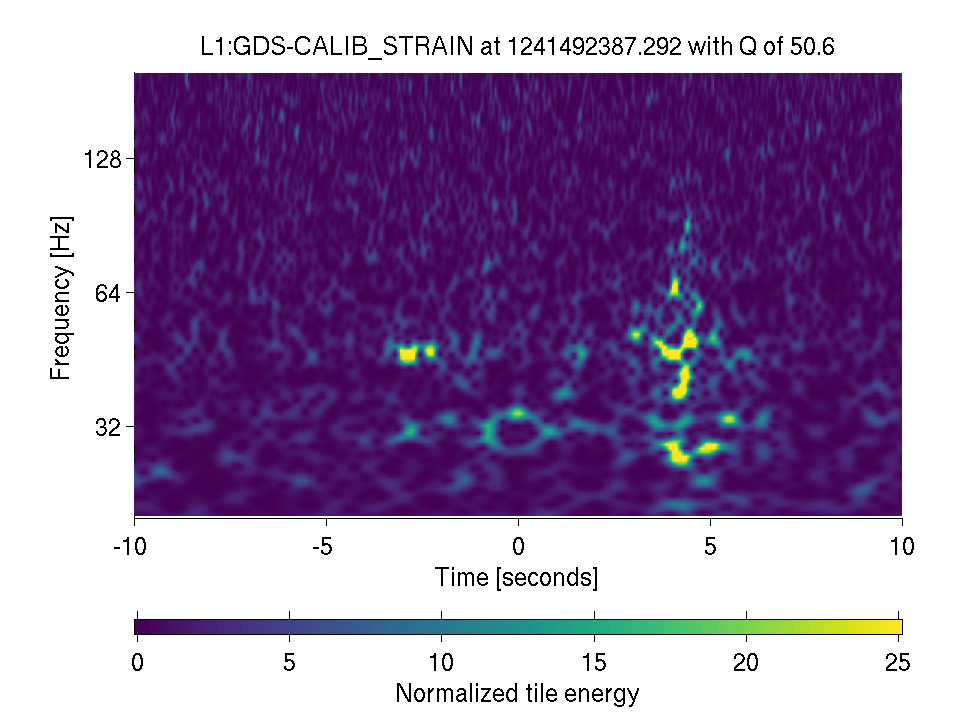
\includegraphics[width=0.49\textwidth]{figures/noise-studies/evaluation-thunder-strain.png}
	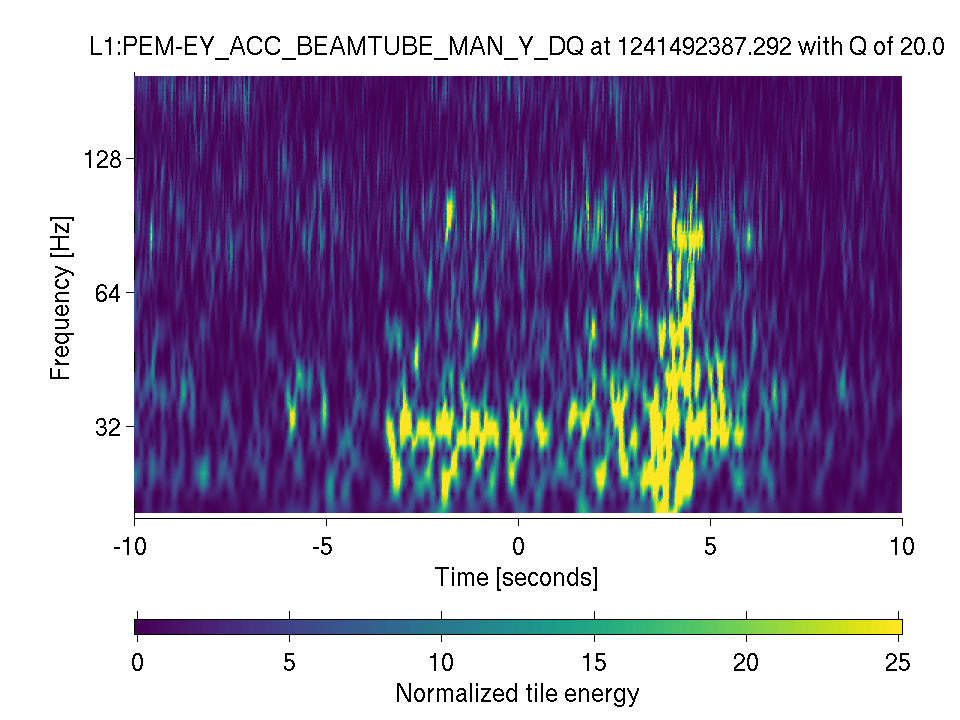
\includegraphics[width=0.49\textwidth]{figures/noise-studies/evaluation-thunder-acc.png}
	\caption{Constant-Q transforms of the GW strain channel (left) and an accelerometer (right) during thunder noise at LLO.}
	\label{fig:evaluation-thunder}
\end{figure}

Helicopter flyovers can produce narrow-band features up to tens of seconds long at harmonics of the main helicopter rotor frequency.
These are reported by site operators if they are loud enough to be heard even within the observatory buildings.
At each site, three flyovers were reporting during O3.
Table~\ref{tab:evaluation-helicopter} presents the noise estimates from coupling functions for various sensors during these events~\citep{alog_helicopter}.
One of the events at LLO was omitted because no excess noise was visible in DARM spectrograms.
For each flyover, the sensor with the highest projection in DARM is reported.
The last column shows the ratio between the estimated projection amplitude and the actual amplitude, confirming that coupling functions can predict the amplitudes of lines produced by helicopter flyovers to within a factor of two in most cases.

\begin{table}
	\caption{\label{tab:evaluation-helicopter}
	Noise projections for five helicopter flyovers at the LIGO detectors.}
	\begin{tabular}{|c c c c|}
		\hline
		& Frequency & Channel & Estimated noise / \\
		& [Hz] & & Actual noise \\
		\hline
		\multicolumn{4}{|c|}{Observatory: LHO \hskip 2em Time: 2019-05-09 21:30 UTC}\\
		\hline
		& 27 & \verb|H1:PEM-CS_ACC_HAM6_OMC_Y_DQ| & 0.7 \\
		& 27 & \verb|H1:PEM-EY_ACC_BSC10_ETMY_X_DQ| & 0.5 (upper limit) \\
		& 90-100 & \verb|H1:PEM-CS_ACC_HAM6_OMC_X_DQ| & 0.8 \\
		& 90-100 & \verb|H1:PEM-EY_ACC_BSC10_ETMY_X_DQ| & 0.8 (upper limit) \\
		\hline
		\multicolumn{4}{|c|}{Observatory: LHO \hskip 2em Time: 2019-05-21 03:11 UTC}\\
		\hline
		& 26 & \verb|H1:PEM-CS_ACC_HAM6_OMC_Y_DQ| & 0.4 \\
		& 39 & \verb|H1:PEM-CS_ACC_HAM6_OMC_Y_DQ| & 1.4 \\
		& 52 & \verb|H1:PEM-CS_ACC_HAM6_OMC_X_DQ| & 0.3 \\
		& 75 & \verb|H1:PEM-CS_ACC_HAM6_OMC_X_DQ| & 0.4 \\
		\hline
		\multicolumn{4}{|c|}{Observatory: LHO \hskip 5em Time: 2019-06-08 17:24 UTC}\\
		\hline
		& 33-40 & \verb|H1:PEM-CS_ACC_HAM6VAC_SEPTUM_Y_DQ| & 1.8 \\
		\hline
		\multicolumn{4}{|c|}{Observatory: LLO \hskip 5em Time: 2019-09-02 17:34 UTC}\\
		\hline
		& 70-80 & \verb|L1:PEM-CS_ACC_HAM6_OMC_X_DQ| & 2 \\
		\hline
		\multicolumn{4}{|c|}{Observatory: LLO \hskip 5em Time: 2020-01-22 22:25 UTC}\\
		\hline
		& 40-44 & \verb|L1:PEM-CS_ACC_HAM6_OMC_X_DQ| & 0.6 \\
		& 90-95 & \verb|L1:PEM-CS_ACC_HAM6VAC_SEPTUM_Y_DQ| & 1.8 \\
		\hline
	\end{tabular}
\end{table}

Long-duration noise due to vibrations from rain and the building \ac{HVAC} is also well characterized by coupling functions at \ac{LHO}~\citep{alog_rain, alog_hvac_coupling}.

\section{Vibrational noise studies during O3}\label{sec:vib}

\begin{figure}
	\centering
	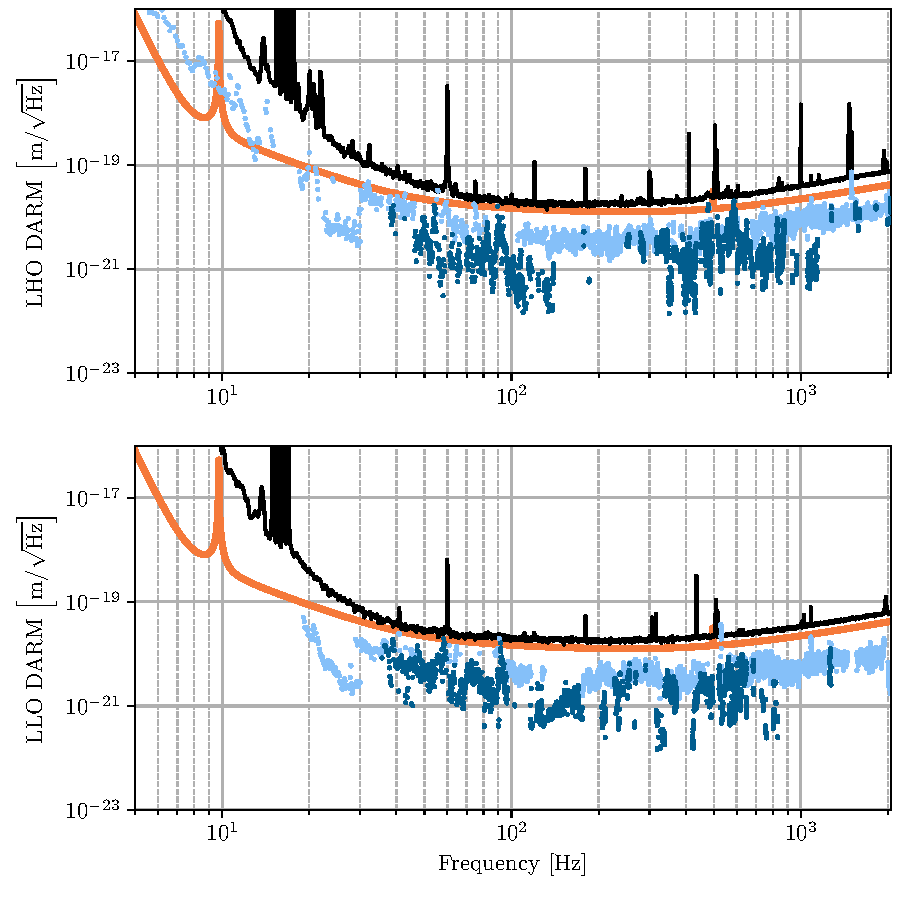
\includegraphics{figures/noise-studies/vib-ambient.pdf}
	\caption
	[DARM noise from all \textit{vibrational} coupling sources at LHO (top) and LLO (bottom).]
	{DARM noise from all \textit{vibrational} coupling sources at LHO (top) and LLO (bottom).
	 Dark blue dots represent measurements, while light blue dots represent upper limits.
	 The black and orange curves show the O3 sensitivity and design sensitivity, respectively.
	 }
	\label{fig:vib-ambient}
\end{figure}

Aggregating our coupling measurements made during O3, we arrive at
Figure~\ref{fig:vib-ambient}, the total ambient contribution of vibrational noise sources during \ac{O3}, produced by combining the highest coupling measurements from accelerometers and microphones and computing their ambient noise projections to the DARM channel.
At both observatories, scattered light noise dominates at low frequency (below 100\,Hz): at the output arm at LHO and at ETMY at LLO.
At higher frequencies the input beam jitter noise dominates.
The physical mechanisms behind these effects were described in Section~\ref{sec:noise-sources}.


\subsection{Scattered light at the HAM5/6 septum}\label{sec:vib-septum}

At \ac{LHO}, investigations throughout \ac{O3} showed that scattering noise at the output arm produces noise near the detector noise background in the frequency range of 38--100\,Hz.
The sensors with the highest ambient projections in this band were accelerometers located on the HAM5 and HAM6 vacuum chambers, which contain the \ac{GW} channel readout, as well as the optics of the output mode cleaner, squeezed light system, and signal recycling cavity.
The coupling was excited most strongly by injections around the output arm, but acoustic noise produced as far as the Y-arm manifold $\approx 50$\,m away produced excess noise in \ac{DARM}.
Figure~\ref{fig:vib-septum-shaker} shows shaker injections performed at the HAM5/6 area.
Mechanical resonances in the vacuum chamber structure alter the frequency content of the injection signal as it propagates, so the sensitivity of the detector to the shaker injections is not uniform but rather characterized by various peaks and troughs.
The estimated ambient noise levels of the worst of these peaks reaches within a factor of two below the DARM background in the 50-60\,Hz and 80-100\,Hz bands, higher than observed by other corner station shaker injections.

\begin{figure}[htb]
	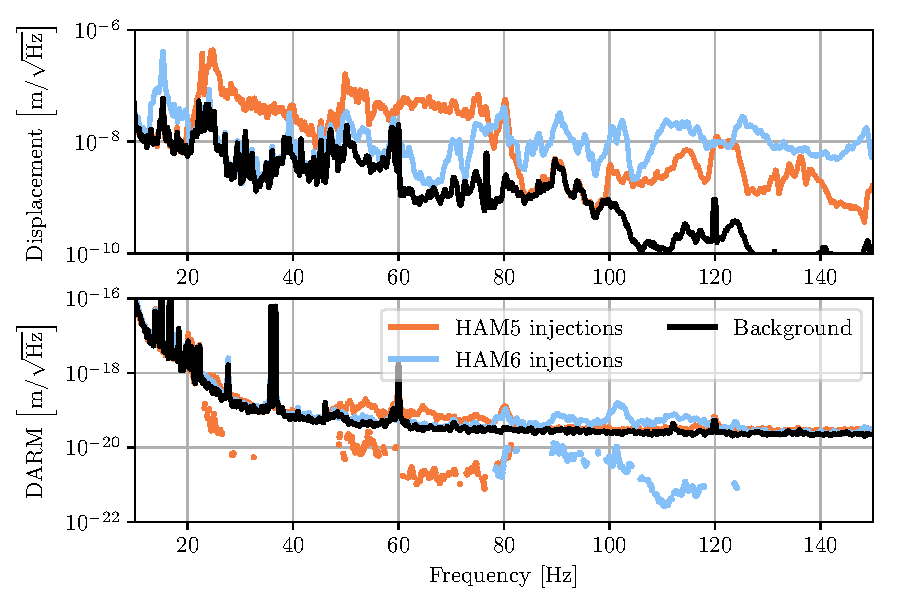
\includegraphics{figures/noise-studies/vib-septum-shaker.pdf}
	\caption[Spectra of shaker injections exciting scattered light noise at the LHO output arm.]
	{Spectra of shaker injections exciting scattered light noise at the LHO output arm.
	 Top: Injections observed by the HAM5/6 septum accelerometer, stitched together from multiple bandpassed injections (each covering a 20-Hz range).
	 Bottom: DARM responses to the injections (solid lines) and estimated ambients from coupling functions in dots.}
	\label{fig:vib-septum-shaker}
\end{figure}

A more thorough investigation was required to localize the exact scattering surface.
We carried out impulse injections, as described in Section~\ref{sec:injections-vib-impulse}, at 37 locations throughout the corner station, including a number of spots on the chamber walls and doors of HAM5 and HAM6.
Figure~\ref{fig:vib-impulse} shows time series and spectrograms the \ac{GW} channel and in various output optics accelerometers during a single impulse injection performed in the HAM5/6 area.
Multiple sensors observe an impulse time-of-arrival matching that of the \ac{GW} channel, but repeating the injection from several other locations rules out sensors that do not match it consistently across multiple injections.
In this case we find that the septum (separating the HAM5 and HAM6 chambers) accelerometer signal matches the \ac{DARM} signal most consistently.
The accompanying spectrograms of the same impulse injection for \ac{DARM} and the three sensors with the closest matching time-of-arrival to that of \ac{DARM} reveal similarities between the frequency structure of the septum accelerometer signal and that of \ac{DARM}.


\begin{figure}[htb]
	\centering
	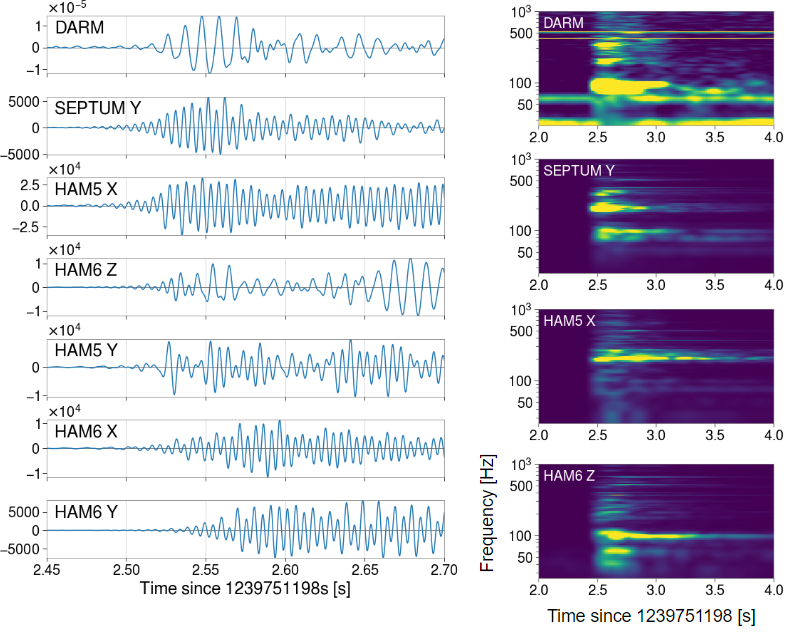
\includegraphics[width=\textwidth]{figures/noise-studies/vib-impulse.png}
	\caption{
		Time series (left) and spectrograms (right) of a vibrational impulse injection produced at the output arm of the LHO detector.}
	\label{fig:vib-impulse}
\end{figure}

Additionally, we performed a series of beating-shakers injections during the commissioning break as described in Section~\ref{sec:injections-vib-beats}, attaching the large and small shakers to the HAM5/6 chamber doors, the outside of the septum itself, and the chamber roofs.
We injected at 100, 200, and 400\,Hz, each time with $\delta f = 100.01$\,Hz and observing for about five minutes.
Due to a metal scaffolding structure placed around the chambers for commissioning work we were limited in our ability to produce strong enough signals to give a clear beat envelope.
Nevertheless these injections did not rule out the septum as a coupling site.

The septum wall is a physically likely coupling site because it is highly reflective, exhibits more ambient motion than other surfaces on the HAM chambers, and stands perpendicular to the path of the interferometer beam, which passes through it via a glass window.
This window was particularly suspected to be the culprit and was replaced during the commissioning break in order to eliminate the scattered beam.
Follow-up measurements, however, show no significant changes in the coupling between the start of O3 and the commissioning break (Figure~\ref{fig:vib-septum-midrun}), suggesting that perhaps the solid septum wall itself is the scattering surface.

\begin{figure}[htb]
	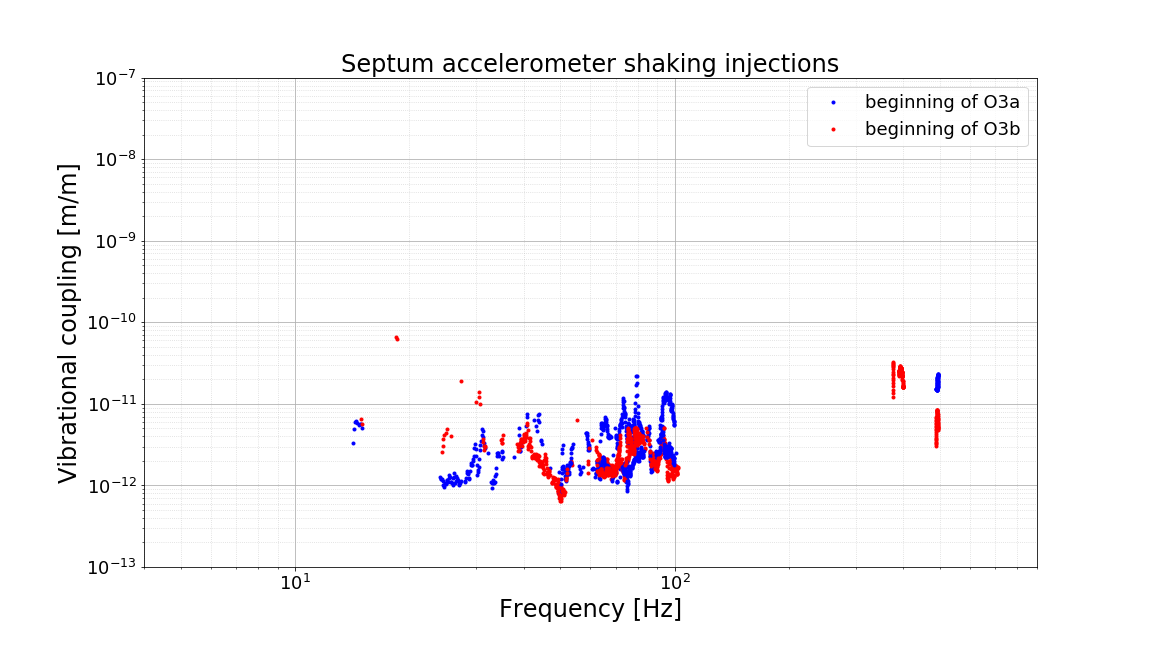
\includegraphics[width=\textwidth]{figures/noise-studies/vib-septum-midrun.png}
	\caption{Change in HAM5/6 vibrational coupling before and after the replacement of the septum window.}
	\label{fig:vib-septum-midrun}
\end{figure}

The plan for post-O3 upgrades was to install light baffles, surfaces with low reflectivity, around the septum to block stray light from hitting the wall.
More recent measurements suggest that even this has not mitigated coupling, however.
This means that the window is indeed the coupling site but that a higher-quality window is not sufficient to eliminate the scattering, so the window must be entirely removed.
This has been done at LLO with preliminary analyses showing significant noise reduction.

The investigation on the septum coupling will continue on the road towards O4.
The results of this investigation and the vibrational noise budget measurements have made it clear that localizing and mitigating coupling due to scattered light beams will be crucial to reaching the design sensitivity of Advanced LIGO.



\subsection{Search for the source of a 48-Hz peak}\label{sec:vib-48hz}

During O3a, a 48-Hz peak with no known source was visible in the DARM spectrum.
This peak often fluctuated in amplitude on the time scale of minutes.
During the pre-O3 injections, we observed that this noise signal was amplified by many vibrational injections in the corner station, especially the input arm acoustic speaker injections (Figure~\ref{fig:vib-48hz-injection}).
Follow-up impulse injections revealed that it was likely near the vertex, potentially pointing to a scattered light source in one of the beam splitter chambers or in HAM3.

\begin{figure}[htb]
	\centering
	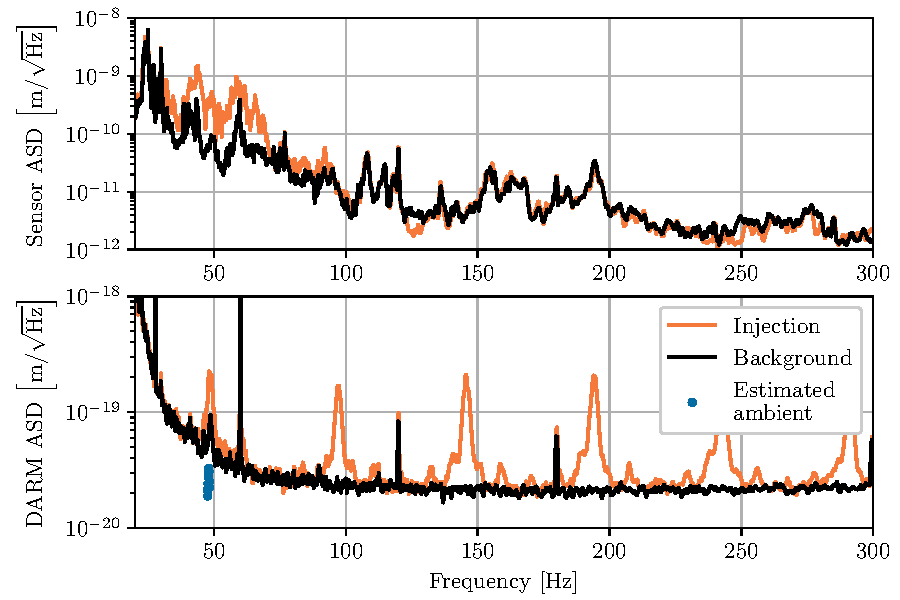
\includegraphics[width=\textwidth]{figures/noise-studies/vib-48hz-injection.pdf}
	\caption{
		ASD of a vibrational injection at the LHO input arm exciting a 48-Hz resonance feature in DARM.}
	\label{fig:vib-48hz-injection}
\end{figure}

Beating-shakers injections were then used to localize the coupling site.
The shakers were injecting from different locations near the input arm and vertex.
One shaker injected at 48\,Hz and the other at 48.01\,Hz.
Figure~\ref{fig:vib-beat-spectrograms} shows spectrograms of the injection signals measured by DARM and by various nearby accelerometers.
The Y-axes of the spectrograms are centered along at 48\,Hz and show the combined signal in each sensor modulating at the beat frequency (0.01\,Hz).
This set of spectrograms suggests that the accelerometers on the \ac{ITM} chambers and the Y-axis HAM2 accelerometer are likely not close to the true coupling location, since the beat envelopes have the greatest phase offset from the beat envelope in the \ac{DARM} response.

\begin{figure}[htb]
	\centering
	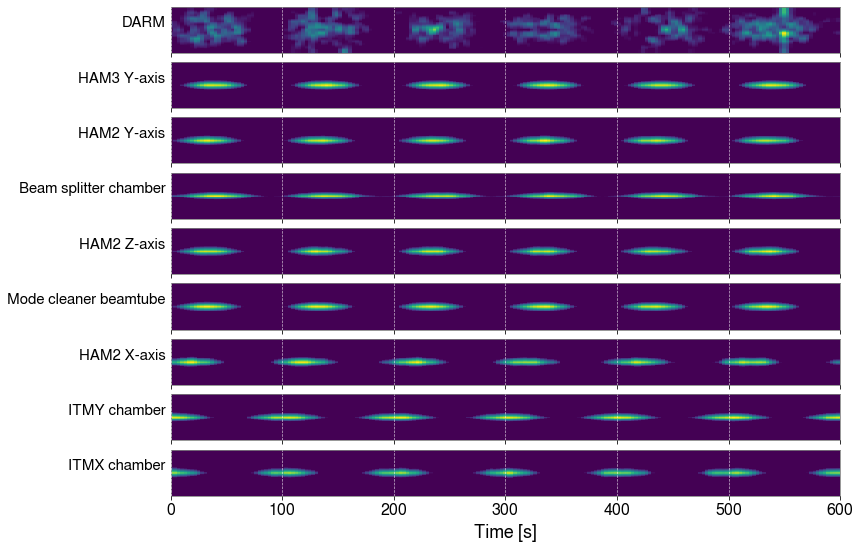
\includegraphics[width=\textwidth]{figures/noise-studies/vib-beat-spectrograms.png}
	\caption{
		Spectrograms of DARM and various accelerometers near the input arm and beam splitter showing a beating-shakers injection at 48\,Hz.}
	\label{fig:vib-beat-spectrograms}
\end{figure}

Multiple other injections were made (not shown here) with varying shaker locations in order to rule out other sensors until the most likely candidate remaining was the HAM3 Y-axis accelerometer.
Black glass was used to block scattered light at this location and the peak was eliminated for the second half of the O3 observation run.
% Figure~\ref{fig:vib-48hz} shows the noise reduction in the \ac{GW} channel after the light scattering was mitigated.

% \begin{figure}[h]
% 	\centering
% 	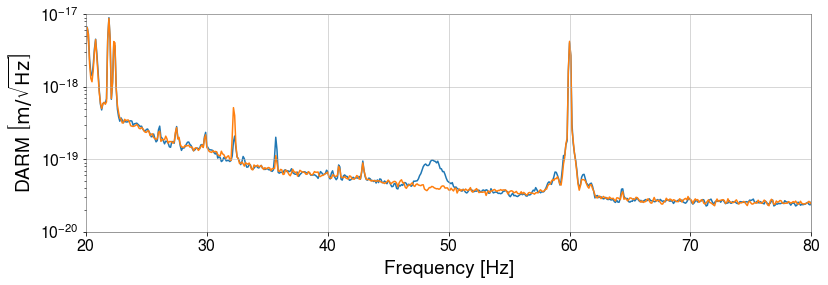
\includegraphics[width=0.9\textwidth]{figures/noise-studies/vib-48Hz.png}
% 	\caption{LHO DARM spectrum before and after mitigation of the 48-Hz peak.}
% 	\label{fig:vib-48hz}
% \end{figure}

\subsection{Input beam jitter}\label{sec:vib-jitter}

Jitter noise was a dominant noise source for both detectors in the hundreds of Hertz frequency range.
The impact was much greater at LHO than at LLO.
Around 480\,Hz, a peak associated with jitter noise could be seen in the LHO DARM spectrum.
It was hypothesized that the higher coupling at LHO was due to a point absorber that was identified on the Y-arm \ac{ITM}.
Point absorbers are defects usually less than a millimeter across found in the test mass coatings.
They are heated by the intense laser power in the Fabry-P\'erot arm cavities, deforming the test mass and increasing the cavity optical loss.
As discussed in Section~\ref{sec:noise-sources}, such defects enhance the coupling of jitter noise since they introduce an asymmetry between the arms.

In December 2020, the affected ITM was replaced with a new one, as part of the upgrades for \ac{O4}.
Thus far no point absorbers have been found on the new test mass.
Jitter coupling functions measured some months later show a dramatic order-of-magnitude reduction compared to the O3 results (Figure~\ref{fig:vib-jitter}).
The ambient noise contribution is now roughly equivalent to that of LLO.

\begin{figure}[htb]
	\centering
	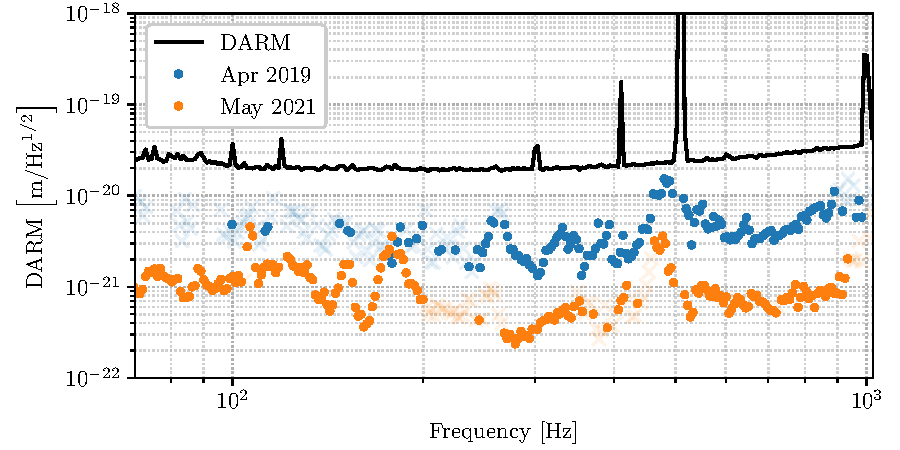
\includegraphics{figures/noise-studies/noise-jitter.pdf}
	\caption{Improvement in jitter coupling at LHO after test mass replacement.}
	\label{fig:vib-jitter}
\end{figure}

Although point absorbers can be avoided by offsetting the beam spot on the test mass, the only perfect solution is to completely change out the test mass.
Therefore we these jitter coupling measurements emphasize the importance of addressing the issue of point absorbers as soon as possible.
The existence of just one point absorber on any of the test masses enhances jitter coupling to the point of introducing excess DARM noise, requiring that we new measurements every time some part of the input optics changes.

\section{Magnetic noise studies during O3}\label{sec:mag}

\begin{figure}
	\centering
	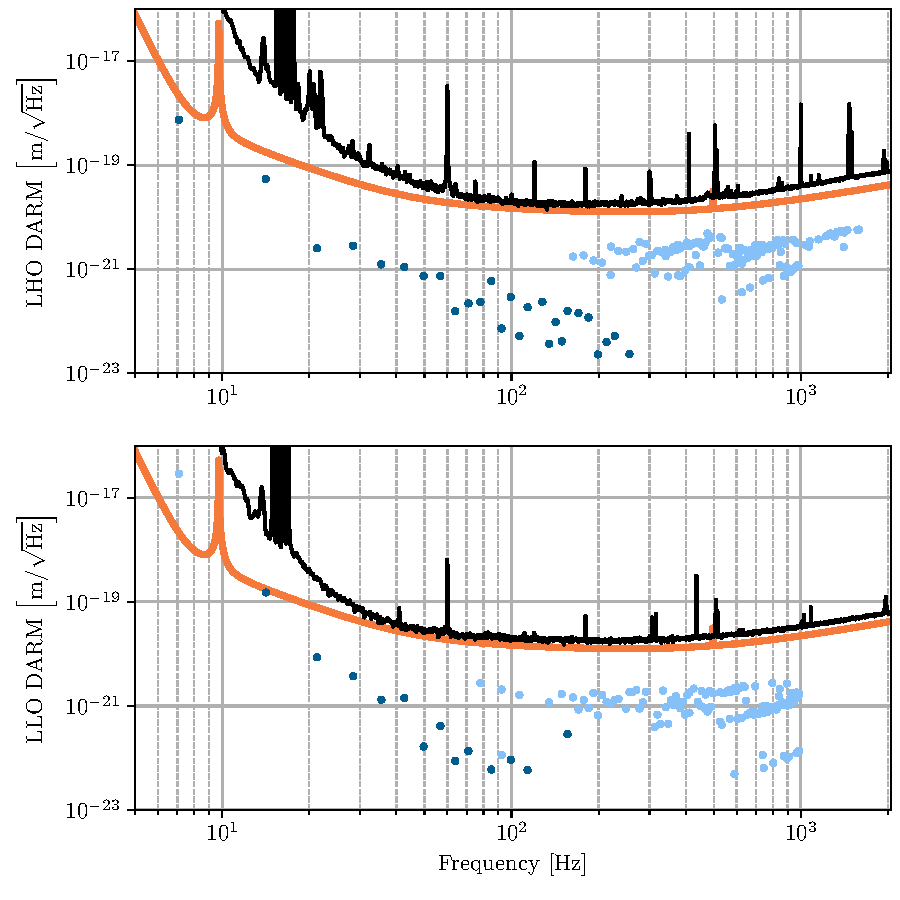
\includegraphics{figures/noise-studies/mag-ambient.pdf}
	\caption
	[DARM noise from all \textit{magnetic} coupling sources at LHO (top) and LLO (bottom).]
	{DARM noise from all \textit{magnetic} coupling sources at LHO (top) and LLO (bottom).
	 Dark blue dots represent measurements, while light blue dots represent upper limits.
	 The black and orange curves show the O3 sensitivity and design sensitivity, respectively.
	 }
	\label{fig:mag-ambient}
\end{figure}

Figure~\ref{fig:mag-ambient} shows the magnetic noise budget produced from coupling functions for all magnetometers for both LIGO observatories.
Magnetic injections in previous runs suggested that coupling to permanent magnets in the suspension system could prevent \ac{LIGO} from reaching design sensitivity in the 10-20\,Hz regions~\citep{Schofield_2013}.
While the test mass actuator is electrostatic and not magnetic (as in \ac{iLIGO}), a number of permanent magnets were used in the suspensions, including for actuation in the first three of the four levels of the isolation chain and for eddy current damping.
The greatest number of permanent magnets were in the eddy current damping arrays and these were removed.
Nevertheless, the current noise budget shows that ambient fields are still predicted to produce noise at a level close or even equal to the design sensitivity in the 10-20\,Hz range (Figure~\ref{fig:mag-ambient}).
Thus low-frequency noise from permanent magnet coupling may need to be revisited in future runs.

At higher frequencies, generally above about 30\,Hz, the dominant magnetic coupling appears to be through induction of currents in cables and at connectors, mainly to actuator cabling and other cabling in the control system.
Mitigation of coupling to cables and connectors has required a continuing program of monitoring coupling since cables are often disconnected and reconnected during runs as electronics are replaced for problems or upgrades.
This program consists of making weekly, broadband magnetic field injections using the large wall-mounted coils described in Section~\ref{sec:injections-magnetic}.
Since the injections are scheduled for every Tuesday morning before the routine detector maintenance period, the interferometer may or may not be in a locked state at the time, so an injections were not always performed.

\begin{figure}
	\centering
	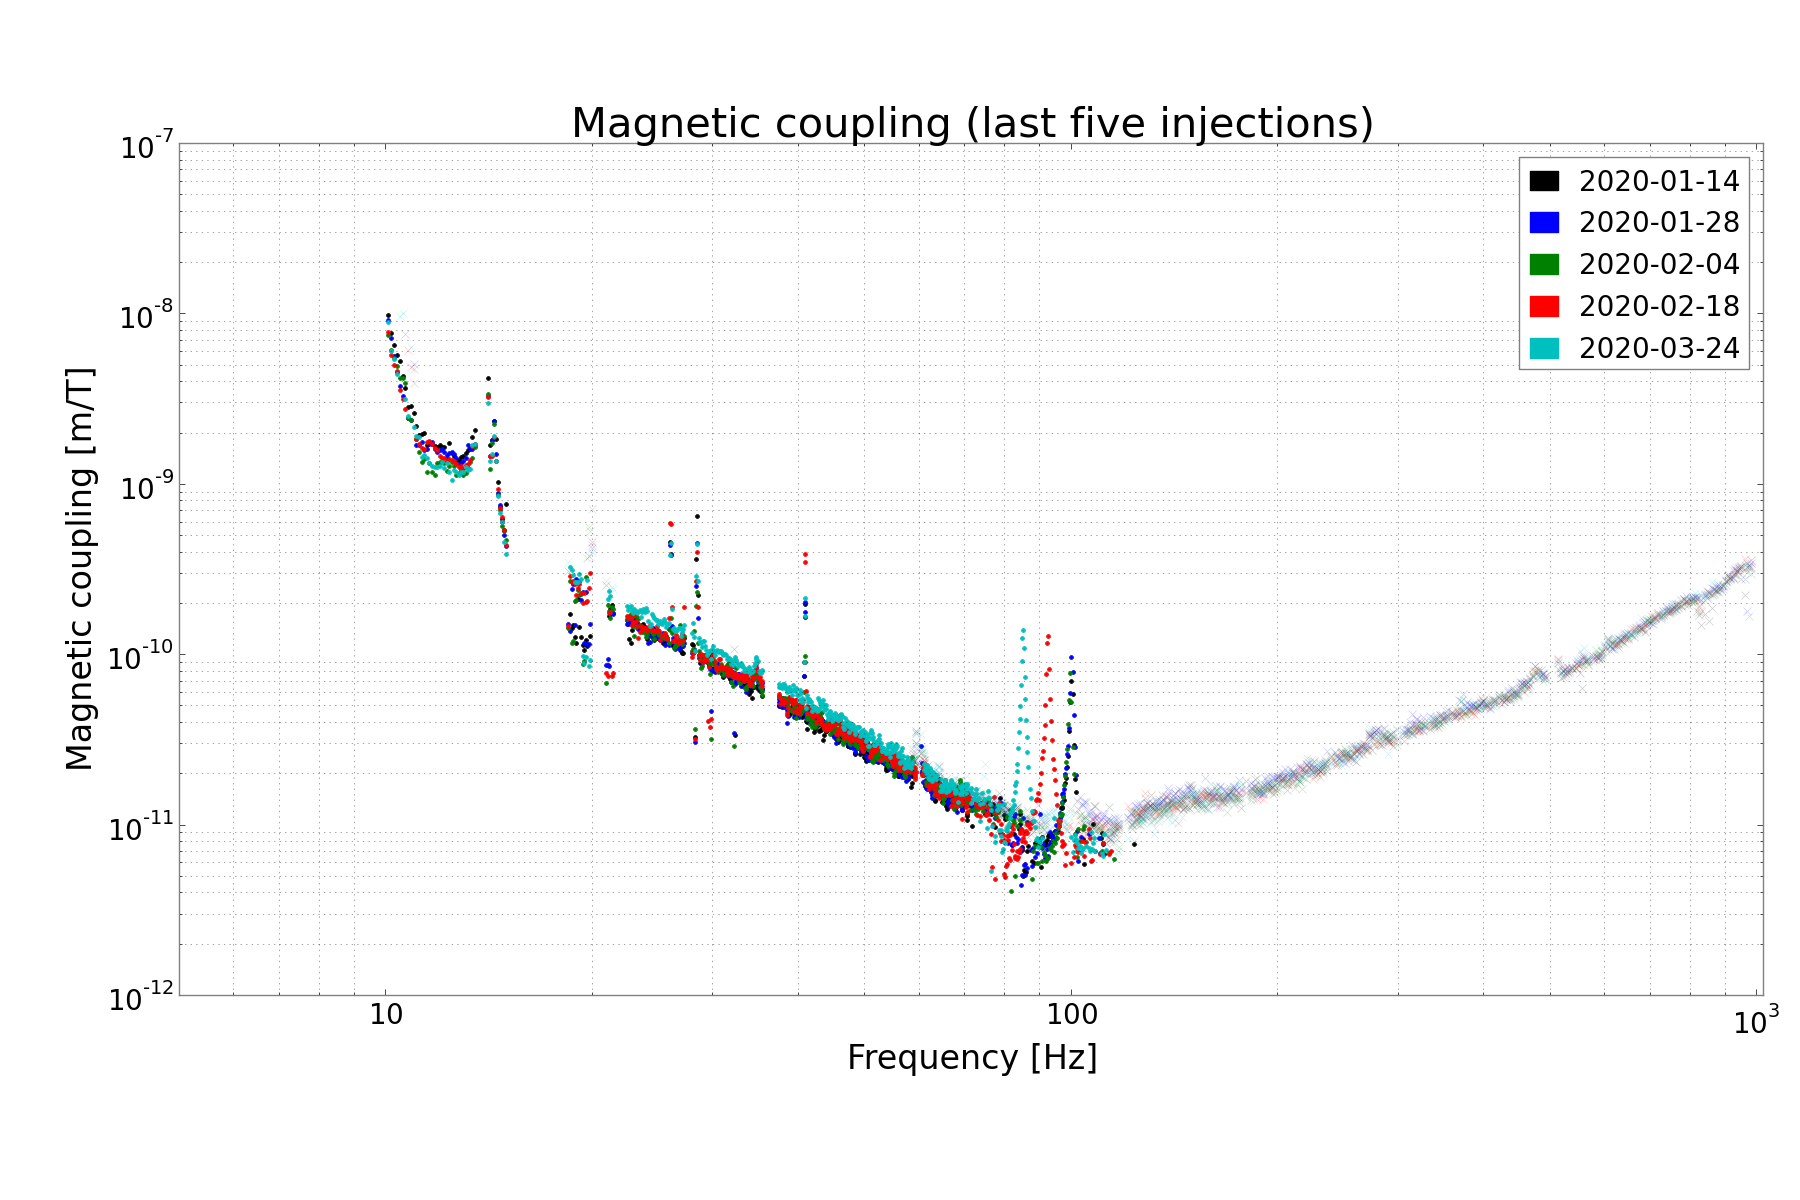
\includegraphics[width=0.9\textwidth]{figures/noise-studies/mag-weekly-cf.png}
	\caption{
		LHO magnetic coupling measured by the last five wall-mounted coil injections performed in O3.}
	\label{fig:mag-weekly-cf}
\end{figure}

Figures~\ref{fig:mag-weekly-cf}, \ref{fig:mag-weekly-bands}, and \ref{fig:mag-weekly-peaks} are automatically generated every week by the code that analyzes the injections.
The first of these shows magnetic coupling functions measured over the last five weeks for which a broadband injection was performed.
At this point a single injector was implemented at each of the three stations at LHO; the coupling functions show the highest coupling per frequency bin between the three stations.

\begin{figure}
	\centering
	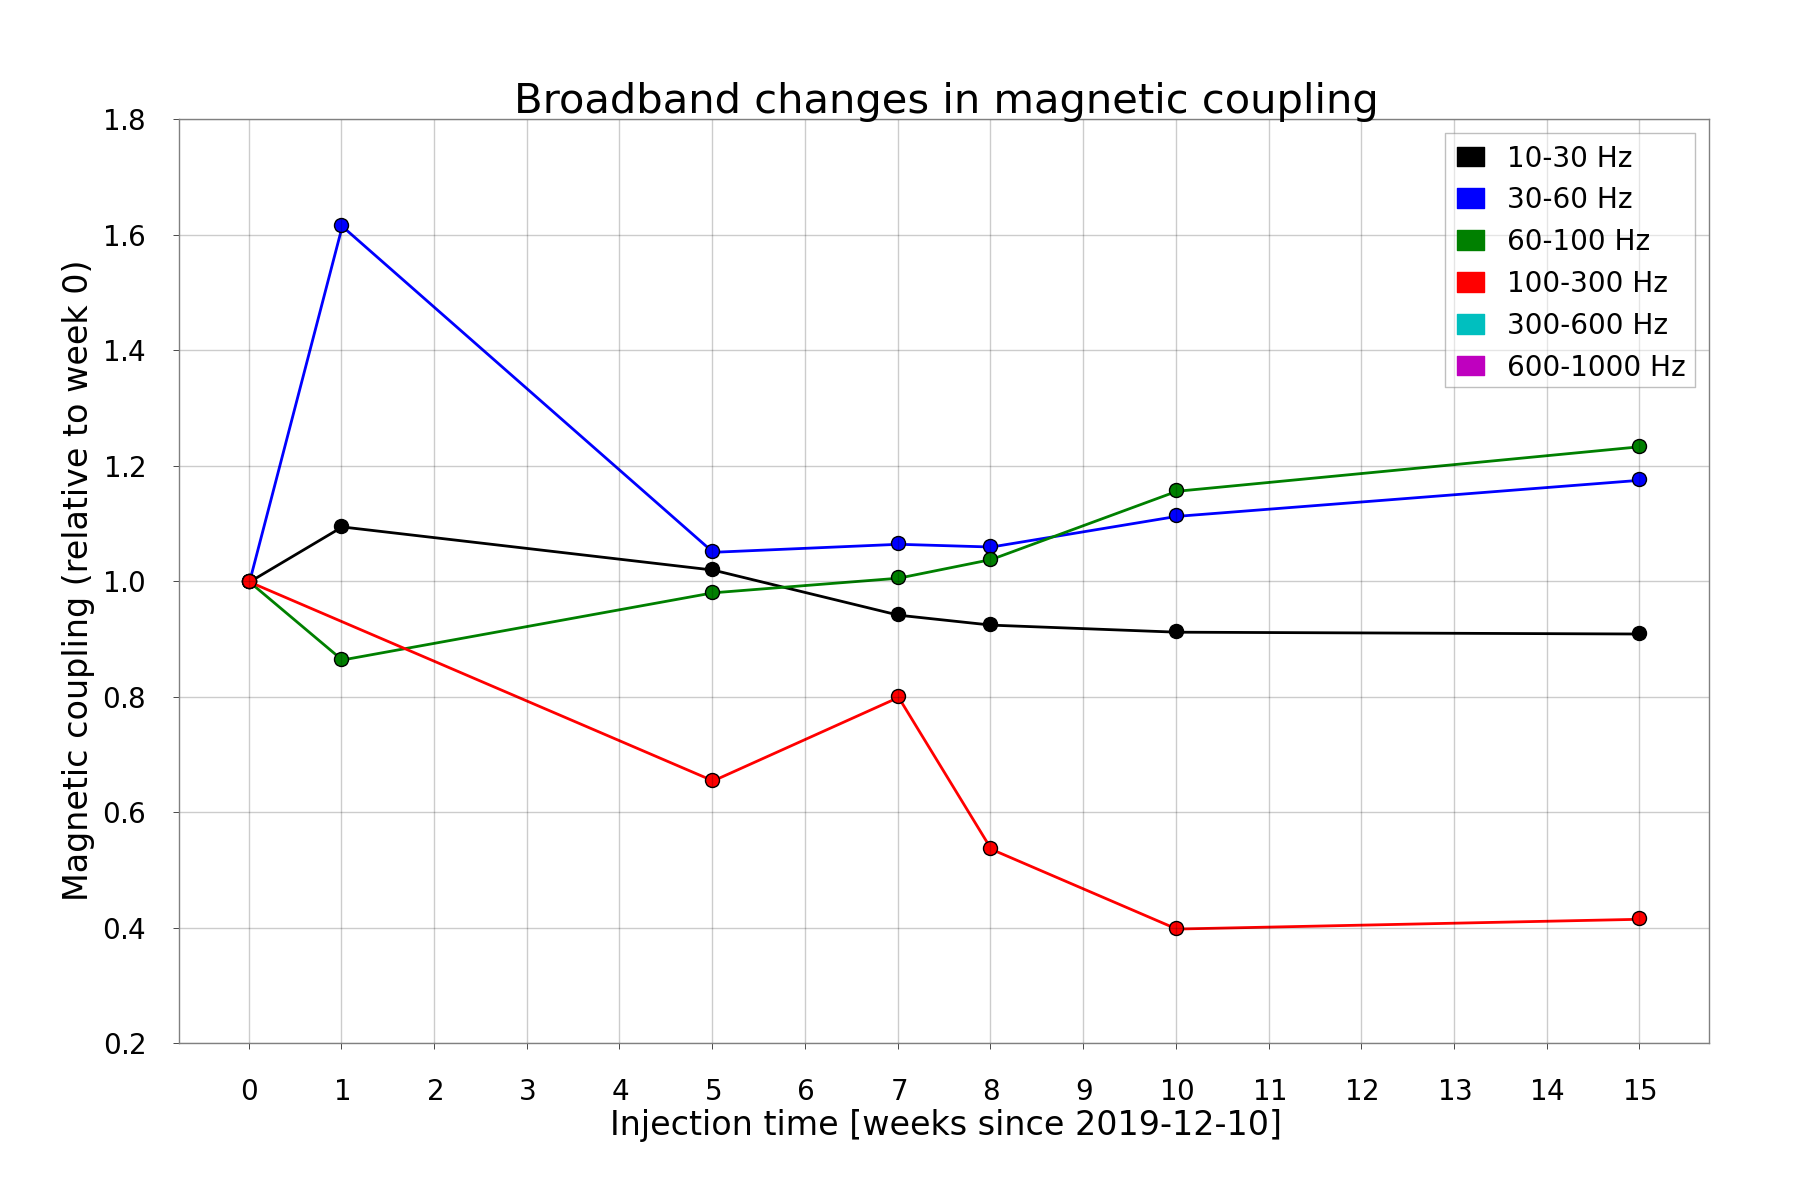
\includegraphics[width=0.9\textwidth]{figures/noise-studies/mag-weekly-bands.png}
	\caption{Time-lines of magnetic coupling changes relative to the start of the observing run.}
	\label{fig:mag-weekly-bands}
\end{figure}

\begin{figure}
	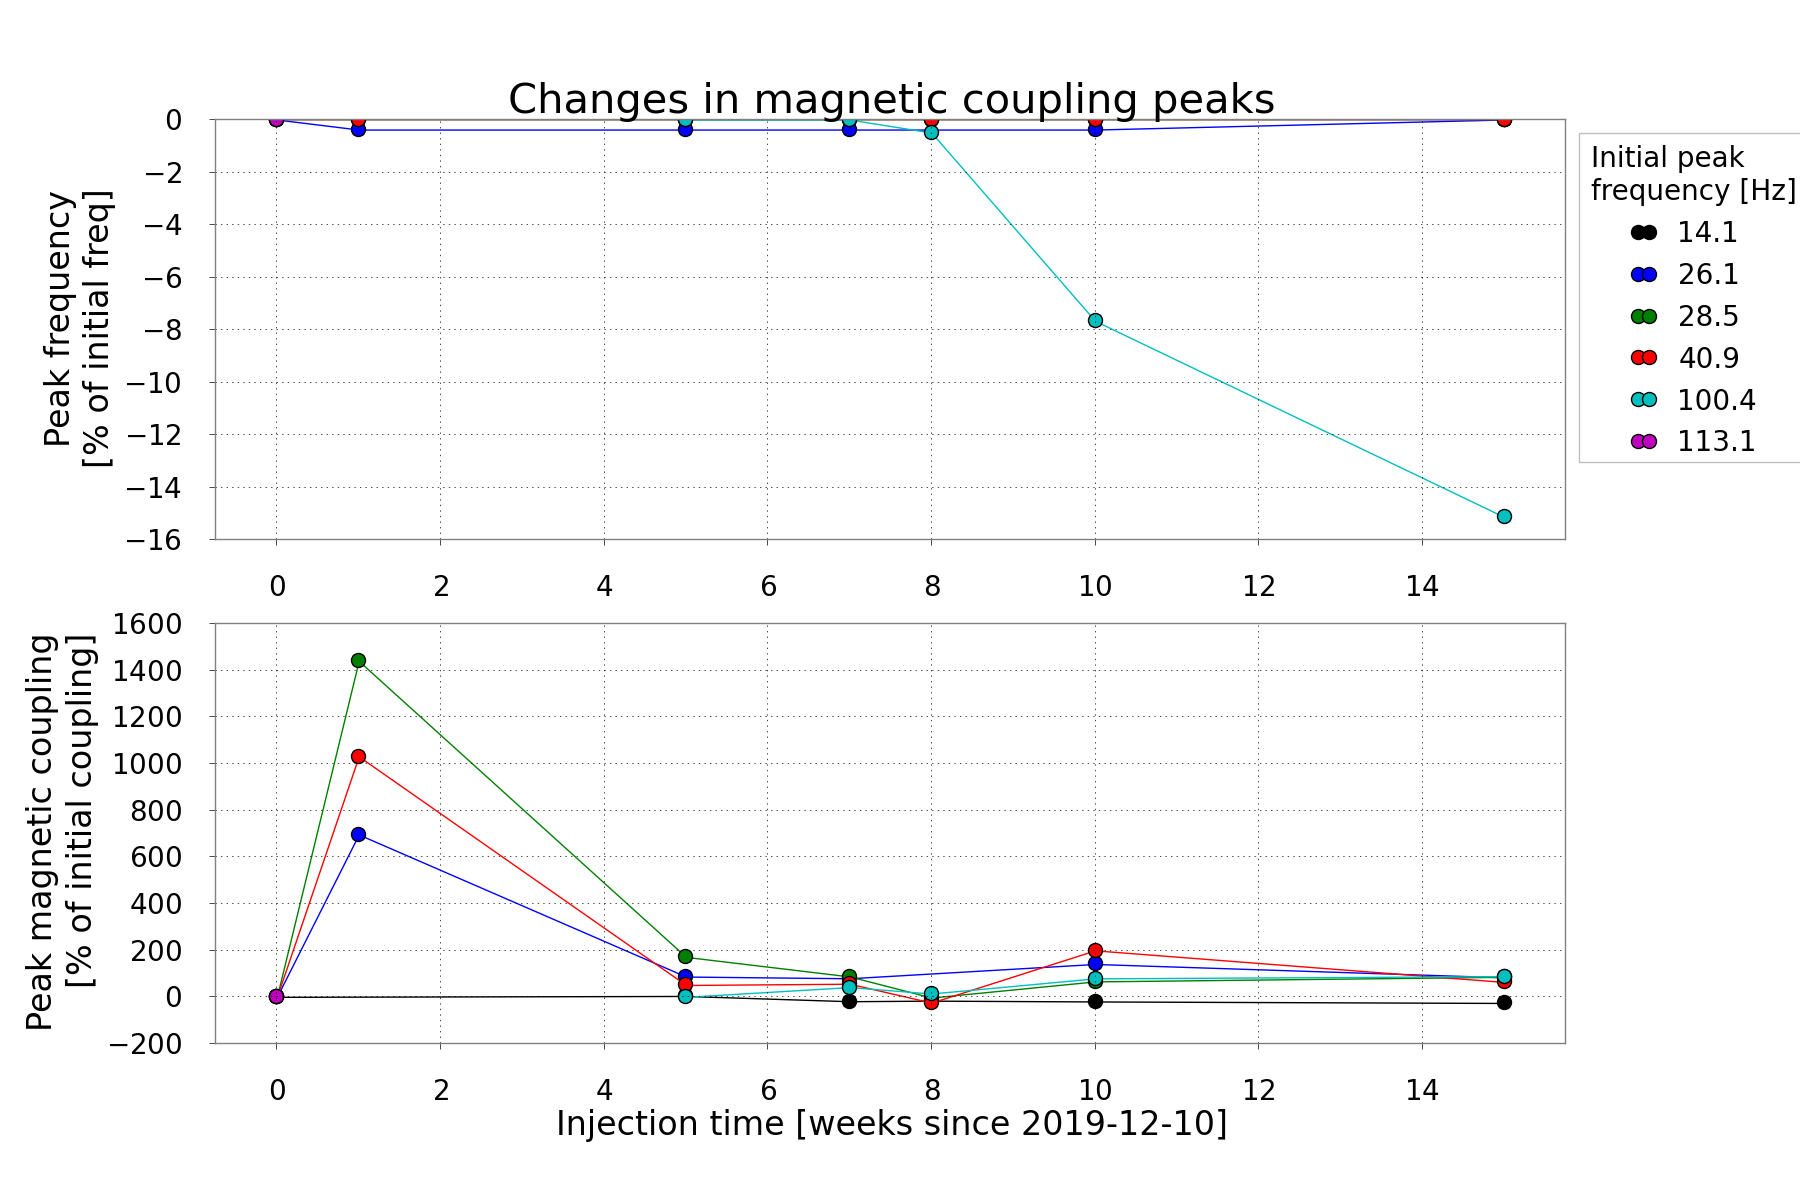
\includegraphics[width=0.9\textwidth]{figures/noise-studies/mag-weekly-peaks.png}
	\caption{Weekly trends in frequency (top) and amplitude (top) of peaks in the magnetic coupling functions.}
	\label{fig:mag-weekly-peaks}
\end{figure}

Changes can be seen in both the broadband and narrowband structure of the coupling function.
Just within these five weeks, the level of broadband coupling varied by as much as a factor of about 1.5.
Since the injection is produced from a same location and at the same amplitude every time, uncertainties due to the injection source as discussed in Section~\ref{sec:uncertainties} do not account for these variations.
Broadband changes over specific frequency ranges tracked over the full course of \ac{O3} (Figure~\ref{fig:mag-weekly-bands}) show significant fluctuations throughout the run.

Furthermore, a large peak in the coupling is seen migrating between 90 and 110\,Hz.
This is precisely the type of feature often missed by comb injections but will be routinely discovered by broadband injections in future observing runs.
Figure~\ref{fig:mag-weekly-peaks} shows frequency and amplitude fluctuations in coupling peaks such as this.
Although the coupling of the $\sim$100\,Hz peak is still well below the level that would produce excess noise in the \ac{GW} channel, its presence gives reason to be concerned that similar peaks could arise in the future that do couple significantly.
These weekly injections would help in identifying when the coupling changed, so instrumentalists can deduce what changes to the electronics may have affected it.

\section{Validation of gravitational wave event candidates}\label{sec:vetting}

In addition to investigating sources of environmental influences, knowledge acquired from environmental studies contributes to the vetting of \ac{GW} event candidates.
Analysis pipelines search the strain data for astrophysical signals.
They are categorized into modeled searches for binary mergers that match the data to template waveforms (e.g. GstLAL~\citep{Cannon_2012} and PyCBC~\citep{Usman_2016}) and unmodeled searches that identify excess energy coherent between multiple detectors (e.g. cWB~\citep{Klimenko_2008}, oLIB~\citep{Lynch_2017}, and BW~\citep{Cornish_2015}).

The template-based modeled searches are incredibly robust to noise transients.
However, environmental noise has the potential to be correlated between detectors by stemming from a common source, such as through electromagnetic signals from distant sources or glitches in GPS-correlated electronics.
The analysis pipelines estimate the false-alarm probabilities for \ac{GW} events based on the background rate of randomly coincident events in the detector network.
They generate background events by time-shifting the data stream of one detector relative to another by time steps much longer than the light travel time between detectors and longer than the duration of \ac{GW} signals.%~\citep{Was_2009}.
This method does not account for the possibility of transients being correlated between the detectors due to a common environmental source.

Environmental noise is also particularly relevant to unmodeled searches. Unlike template-based methods, these searches make minimal assumptions about the signal waveform and rely more heavily on signal correlation between sites.
They are therefore more likely to pick up chance coincidences of environmental transients of various time-frequency morphology.

Furthermore, even if an environmental signal does not account for excess noise in the strain channel during a GW event, it may still impact parameter estimation analyses that infer properties of the GW source.
Most GW events are short in duration, meaning that any chance overlap between an astrophysical signal and a noise artifact, although quite rare, would have a significant impact on these analyses.
In O3, many parameter estimation analyses of GW detections had to limit their frequency ranges to avoid contamination from effects such as scattered light noise.


\subsection{Past methods}

The first observation of a \ac{GW} occurred on 14 Sept 2015~\citep{gw150914}.
The event, a short-duration binary black hole merger designated GW150914, required a number of follow-up investigations to find potential noise sources around the time of the event~\citep{Detchar_2016}.
This included an examination of the status of all \ac{PEM} sensors and any significant signals they observed for possible contamination of the GW signal~\citep{Schofield_150914}.
A few of the \ac{PEM} sensors were not working, but because of redundancy, coverage was sufficient.

Comparisons between constant-Q transform spectrograms~\citep{Chatterji_2004} of all coincident events in environmental sensors to the time-frequency path of the event revealed that no environmental signals had paths similar to the event candidate.
Q-transforms produce a quality-factor-optimized logarithmic tiling of the time-frequency space, making them useful for visualizing transients.
The \acp{SNR} of the matching signals were also compared to that of the event, showing that even if there were overlapping time-frequency paths, none of the environmental signals were large enough to influence the strain data at the \ac{SNR} level of the event, based on multiplying the environmental signals by their respective sensor coupling functions.

The validation process for novel events such as GW150914 also includes redundant checks for global sources of environmental noise.
We use a dedicated cosmic ray detector located below an input test mass at \ac{LHO} to examine any association of cosmic ray showers to excess noise in \ac{DARM}.
We also check external observatories for coronal mass ejections, solar radio signals, geomagnetic signals, and \ac{RF} signals in the detection band as well as higher frequencies.

There was specific concern over a co-incident extremely-high current (504\,kA) lightning strike over Burkina Faso, prompting additional studies of the effects of lightning on the interferometer~\citep{Schofield_lightning}.
Investigations of similar strikes found no effect on the strain data and investigations of closer strikes confirmed that the magnetometers were much more sensitive to lightning strikes than the interferometer was.
In conclusion there was no reason to veto the first detection based on environmental disturbances.

Subsequent detections throughout \ac{O1} and \ac{O2} employed a similar procedure; however the development of the method described in Section~\ref{sec:cf} for producing coupling functions for all sensors expedited the process.
This was especially important for examining environmental noise during GW170817, the first long-duration event detected by \ac{LIGO}~\citep{gw170817, Schofield_170817}.
The longer duration of this event (75\,s) unsurprisingly overlapped with many environmental signals.
Based on the coupling functions for those sensors, several of these environmental events were loud enough (estimated \ac{DARM} signals of up to \ac{SNR}~4) to have contributed to the interferometer readout, but not enough to account for the \ac{GW} signal.
Furthermore, none of them had a time-frequency morphology that correlated with any features in the candidate signal.


\subsection{Automated validation of O3 events}

Since the start of \ac{O3}, most of the procedure described above has been automated in order to handle the increase in detection rate.
The automated vetting is performed by the \code{pemcheck} routine, which is a part of the \ac{DQR}.
When an event is detected by the astrophysical search pipelines, a \ac{DQR} is initiated and assembles a plethora of tasks for assessing the data quality at each observatory during the time of the event.
Among these tasks, an \textit{omega scan pipeline}~\citep{Davis_2021, Chatterji_2004} is used to search for transient noise in all \ac{PEM} sensors in the time window spanning the event candidate.
It does so by producing a Q-transform for each sensor and reporting those in which there is a transient signal with a false-alarm rate below $10^{-3}$\,Hz.
The omega scan also reports the frequency and amplitude of the most significant tile for each sensor.
The \code{pemcheck} in \ac{O3} used the output of the omega scan to estimate each sensor's potential affect on the data quality of the detector.
The coupling function of each sensor was interpolated at the peak frequency and multiplied by the peak amplitude, producing an estimated \ac{DARM} amplitude.

Sensors whose estimated contribution exceed one tenth of the \ac{DARM} background level were flagged for human input, requiring a comparison of the environmental signal morphology to that of the event candidate.
If there was sufficient signal overlap, reviewers may advise that analysts perform some noise removal in the data, such as by gating or filtering out the appropriate time or frequency range, before performing further follow up analyses.
The event could be retracted, if gating or filtering out the environmental contribution would reduce the signal-to-noise ratio of the candidate to a level no longer consistent with a GW detection.

To confirm that PEM sensor coverage was sufficient to make a confident statement regarding environmental contamination, an additional DQR task checked for the most recent output from \ligocam, described in Section~\ref{sec:ligocam}.
This task was used as a supplement to the results reported by \code{pemcheck}.

During \ac{O3}, we confirmed that environmental noise did not account for any of the 74 GW events detected~\citep{gwtc2, gwtc3}.
Some excess noise was always estimated to potentially exist around the events due to the conservative upper limits we set for our coupling functions, but no signal overlap of any environmental transients with GW candidates was seen even for those worst-case upper limit projections.
That said, for most events we cannot rule out the possibility of environmental noise affecting parameter estimation pipelines.


\subsection{Science Case Study of S200114f}

On January 14, 2020, the \ac{cWB} pipeline~\citep{imbh_o3} reported a GW trigger S200114f that was not associated with any triggers from a template-based search pipeline.
It was the highest significance event detected by an unmodeled search alone.
Since this meant the possibility of a non-merger source, a science case study team was put together by the LIGO collaboration to assess the astrophysical nature of the trigger.
Of particular interest was the existence of environmental noise observed by some accelerometers at the LHO output arm.
This was a known source of noise, associated with fan located on the squeezer optics table by HAM6.
Ambient fan motion does not produce noticeable transient signals, but changes in the fan speed cause a vibrational impulse that is much louder than the ambient motion.
In this case a change in the fan speed right at the time of S200114f, producing a second-long glitch at the fan speed of 76\,Hz and at several of its harmonics.
Although the higher harmonics produced more noise, the fundamental frequency was very close to the central frequency of the GW trigger, prompting suspicion that it may have accounted for or at least contributed to the signal SNR.

The nearest sensor observing this noise was an accelerometer mounted on the squeezer table itself.
Table accelerometers are relatively isolated from most acoustic and vibrational injections made at the beginning of an observing run, so only upper limits were available for making initial noise projections.
Follow-up injections were performed soon after that provided much better coverage, and the updated noise projections showed that the expected noise in the strain channel was about an order of magnitude below background levels.
This rejects the possibility that the environmental transient accounts for the LHO detection of S200114f, since the trigger has a significant SNR.
However, the estimated projection for the 152\,Hz harmonic was only a factor of two below background, so we could not rule out the impact of this noise on any parameter estimation that might be attempted on the full \ac{cWB} signal.


\subsection{Event validation in O4}

With the \ac{GW} detection rate expected to increase in \ac{O4}, a more sophisticated and streamlined vetting routine is necessary.
The \ac{DQR} in \ac{O4} will report a p-value for each vetting task, including the \code{pemcheck} task.
In the case of environmental noise vetting, this p-value represents the null-hypothesis probability, i.e. the probability that environmental disturbances are not contaminating the \ac{GW} event signal.
This probability is defined based on the uncertainty of the coupling functions.

Suppose we have measured the coupling for a sensor at a single frequency bin, $C(f_k)$.
As we know systematic uncertainties result in coupling measurements to be log-normally distributed (see Section~\ref{sec:uncertainties-hardware}), we can describe the true coupling with a log-normal distribution with mean $\ln C(f_k)$ and standard deviation $\ln 2$ (corresponding to a factor two uncertainty).
If only an upper limit is available, then the coupling must be equal to or less than the upper limit, so it can be described by a uniform probability distribution between 0 and the upper limit.
Thus multiplying these distributions by the sensor ambient we get a probability distribution for the projected noise level $h_p(f_k)$ in the \ac{GW} channel in terms of $\mu = C(f_k) \cdot X(f_k)$:

\begin{equation}
	P(h_p) = \frac{1}{h_p \sqrt{2\pi} (\ln 2)^2} \exp \left[ -\frac{\ln h_p - (\ln \mu)^2}{2 (\ln 2)^2} \right]
\end{equation}
for measurements and

\begin{equation}
	P(h_p) =
		\begin{cases}
      \frac{1}{CX} & \text{if}\ x < CX\\
      0 & \text{otherwise}
    \end{cases}
\end{equation}
for upper limits.

We can write the probability that the projected noise actually exceeds some \ac{GW} channel background level $h_{\text{bkg}}(f_k)$ based on the corresponding cumulative distribution functions:

\begin{equation}
	P(h_p > h_{\text{bkg}}) =
		\begin{cases}
			1 - \frac{1}{2} \left[ \erf \left( \frac{\ln h_p - \ln \mu}{\sqrt{2} \ln 2} \right) \right] & \text{(measurement)}\\
			1 - \min(1, \frac{h_p}{\mu}), & \text{(upper limit)}
		\end{cases}
\end{equation}

This is computed for every time-frequency pixel of a spectrogram, producing a probability spectrogram image that shows how likely there is to be excess noise within each pixel.
We can then search for the highest probability within pixels that overlap a \ac{GW} transient in order to report the probability that environmental noise in the vicinity of the \ac{PEM} sensor is contaminating the signal of interest.

\begin{figure}
	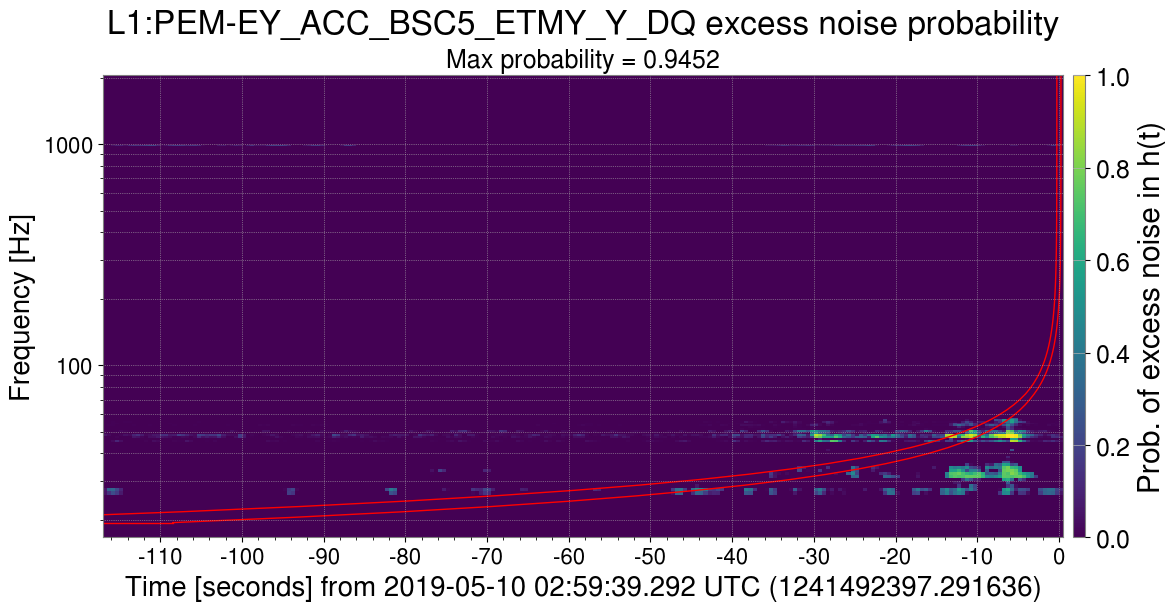
\includegraphics[width=\textwidth]{figures/noise-studies/vetting-spectrogram1.png}
	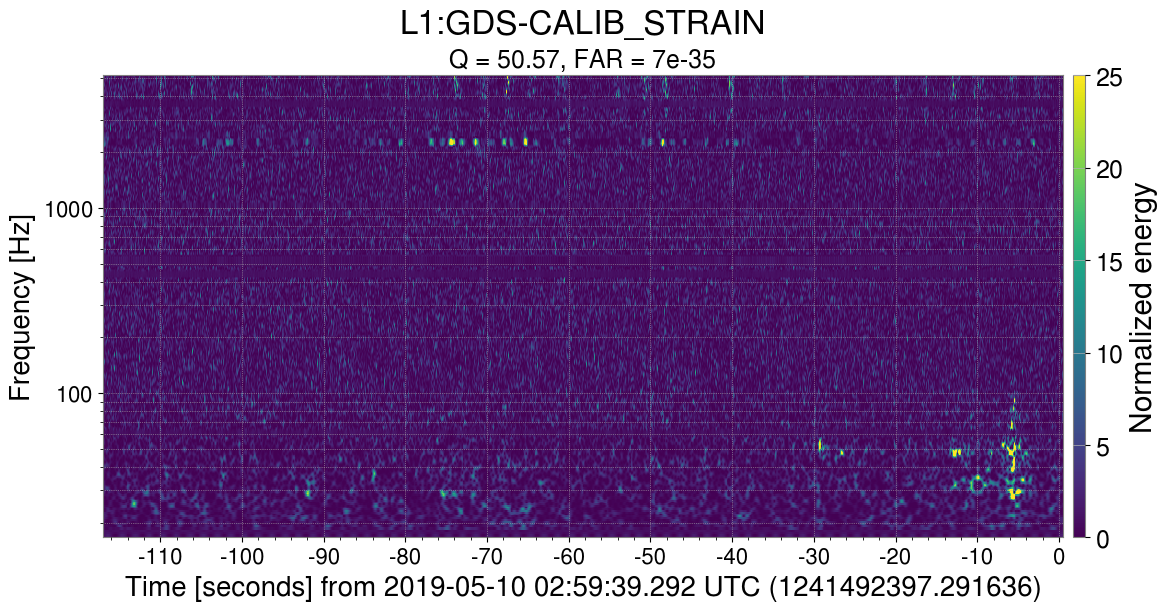
\includegraphics[width=\textwidth]{figures/noise-studies/vetting-spectrogram2.png}
	\caption
	[Probability spectrogram of an ETMY accelerometer at LLO and a constant-Q transform of the GW strain channel]
	{
		Probability spectrogram of an ETMY accelerometer at LLO (top) and a constant-Q transform of the GW strain channel (bottom).
		The red lines show the time-frequency path of GW event candidate S190510g.}
	\label{fig:vetting-spectrograms}
\end{figure}

Figure~\ref{fig:vetting-spectrograms} provides an example of a probability spectrogram output by \code{pemcheck} for an \ac{O3} \ac{GW} event candidate, S190510g.
The candidate signal coincides with scattering noise produced at the \ac{LLO} Y-end station by a thunderstorm.
The coupling projection predicts a peak probability of 0.95, meaning there is an 95\% probability that noise is present in the interferometer overlapping the time-frequency window of the \ac{GW} event.

This algorithm is run on every \ac{PEM} sensor with an available coupling function and the highest probability among all sensors is reported.
We report the p-value of consistency with the null hypothesis as one minus the highest probability, so if a low p-value ($\lesssim$0.1) is reported for a GW event candidate then we cannot rule out the possibility of excess noise contributing to the GW data.
There are still limitations to how well this method can predict the presence of excess noise in the \ac{GW} channel, discussed below.

\subsubsection{Coupling function tuning}

Coupling function projections often overestimate the \ac{GW} background level for a number of reasons.
The most common causes are all linked to the fact that coupling functions can only be measured during extended periods of detector maintenance, usually at the start of an observing run, leaving them vulnerable to becoming outdated as noise sources are introduced, changed, or mitigated.
If a noise source is introduced near a sensor, such as through the installation of new hardware, the sensor ambient can increase dramatically whether or not the noise source actually couples to the \ac{GW} channel.
If the new noise does not couple, then the projection overestimates the detector amplitude, leading to a spurious claim that a \ac{GW} candidate signal may be affected by environmental noise.
Conversely, if an existing noise source is removed or its coupling mechanism mitigated, then the \ac{GW} background drops, potentially below the level of estimated ambient noise projections.

For these reasons, coupling functions must be tuned to account for overestimated noise in the time around an event candidate.
This is done by simply treating background noise in a long stretch of time before the candidate as if it were a new injection.
Rather than re-measuring the coupling function, we can check for frequencies where projections estimate ambient coupling to exceed the \ac{GW} background, dividing the coupling function by the ratio by which it is overestimating.
The result is a coupling function that at most projects noise at background levels.

\begin{figure}
	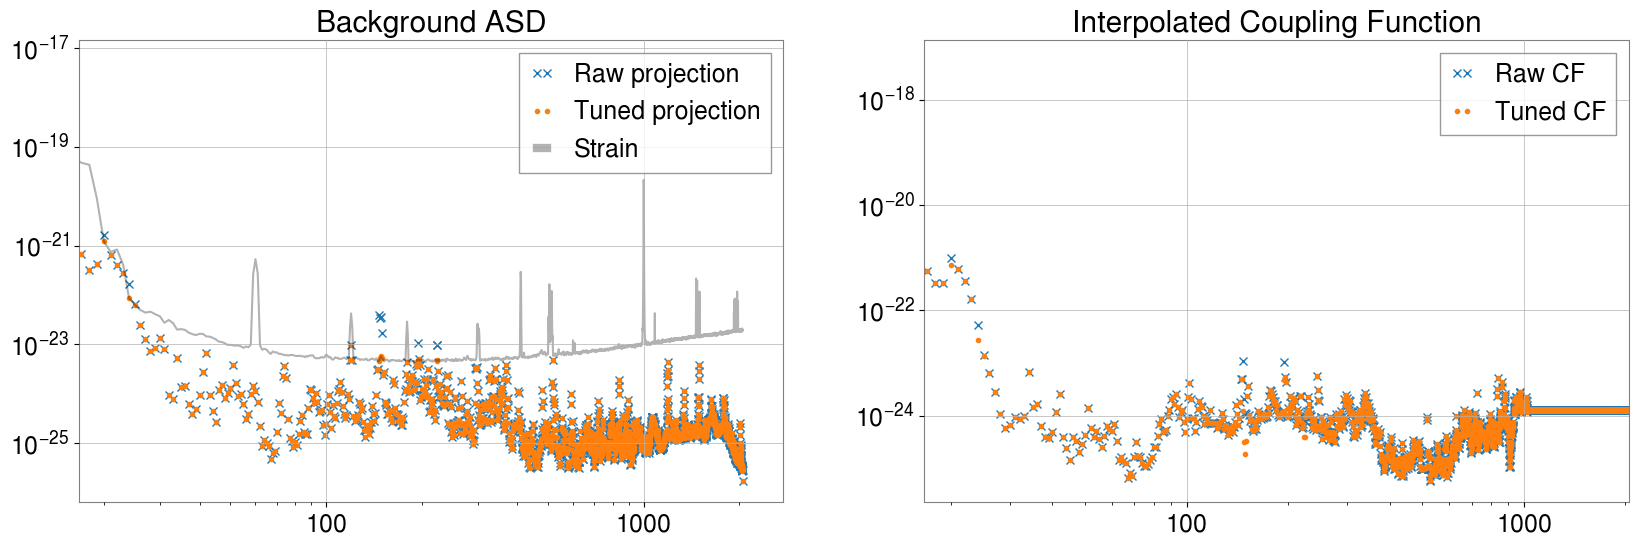
\includegraphics[width=\textwidth]{figures/noise-studies/vetting-tuning1.png}
	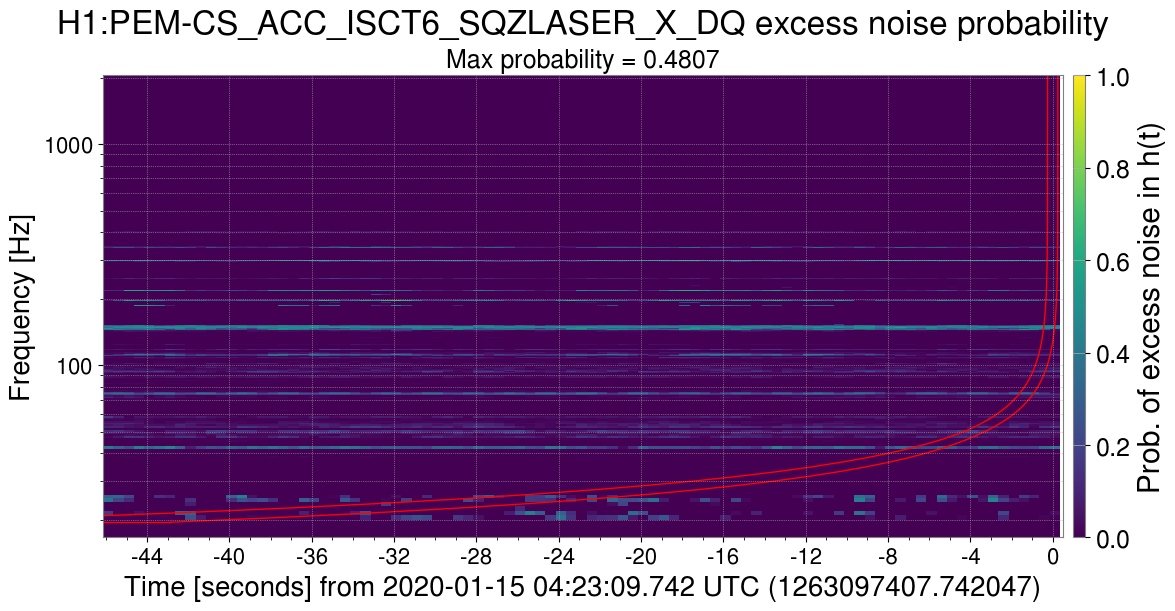
\includegraphics[width=\textwidth]{figures/noise-studies/vetting-tuning2.png}
	\caption
	[Coupling function tuning and the resulting probability spectrogram]
	{
		Coupling function tuning (top) and the resulting probability spectrogram (bottom).}
	\label{fig:vetting-tuning}
\end{figure}

Figure~\ref{fig:vetting-tuning} shows an egregious case of projected noise for an accelerometer on the squeezed light optics table overestimating the strain background amplitude.
The tuning reduces this to match the strain background, and the resulting probability spectrogram does not estimate a significant probability that excess noise is present.


\subsubsection{Grouping nearby sensors}

Even after tuning coupling functions, projections can still be overestimated in the presence of short duration ($\leq$ 1\,s) transients that are not likely to couple based on physical reasons.
Rack magnetometers (placed on the metal racks that hold the various control systems, data acquisitions systems, and power supplies in the electronics rooms) observe the highest rates of localized short-duration transients, routinely picking up magnetic fields from changes in nearby currents.
When these glitches coincide with a \ac{GW} event candidate they predict a probability of excess noise usually above 90\%.
Although the coincident rate is low for typical (\ac{BBH}) events, a long-duration \ac{GW} signal such as a \ac{BNS} will typically overlap with at least a few electronics glitches.

Since coupling functions are only intended to be used for noise sources distant from the sensors, projections from sensors placed close to each other ($\lesssim$ 1\,m) should be highly correlated if the input noise is environmental and not local to the individual sensors.
To incorporate this knowledge, \code{pemcheck} groups together magnetometers in each electronics room; their probability spectrograms are stacked and a pixel-wise minimum is computed to generate a combined group spectrogram.
This suppresses signals that project above the strain background in one magnetometer but not the others, so the projected excess noise probabilities are much lower than any of the peak probabilities reported by the individual sensors.
